\documentclass{beamer}
% The graphics package
\usepackage{graphicx}
% Allows for symbols in lists
\usepackage{amssymb}


%%%%%%%% Title %%%%%%%%%%%%%%%%%%%%%%%%%%%%%%%%%%%%%%%%%%%%%%%%%%%%%%%%%%%%%%%%%
\title{Package Manager}
\subtitle{Team Figjam}
\author{\fontsize{10}{1}\selectfont
        Merrick Heley
        \and
        Tony Lee
        \and
        Nathan Woodrow
        \and
        Steven Eggington
        }
\institute{DECO2800 - Design Computing Studio 2}
\date{9 September 2013}


%%%%%%%% Notes, commands, settings %%%%%%%%%%%%%%%%%%%%%%%%%%%%%%%%%%%%%%%%%%%%%

% Set the theme for the presentation
\usetheme{Frankfurt}

%%%%%%%% Start document %%%%%%%%%%%%%%%%%%%%%%%%%%%%%%%%%%%%%%%%%%%%%%%%%%%%%%%%
\begin{document}

% Title frame
\begin{frame}
    \titlepage
\end{frame}

\section{Introduction} %--------------------------------------------------------
\subsection{}

\begin{frame}
    \frametitle{Background}
    
    Course requires building a game arcade
    \\~\\
    Currently:
    
    \begin{itemize}
        \item   Total rebuild of the client to add games
        \item   Class paths are hard-coded
    \end{itemize}
    
\end{frame}

\begin{frame}
    \frametitle{Context}
    
    How a package manager can improve this
    \begin{itemize}
        \item   Downloadable games
        \item   Dynamic loading
    \end{itemize}
    
\end{frame}

\section{Operation} %-----------------------------------------------------------
\subsection{}

\begin{frame}
    \frametitle{Operational Concept}
    
    Downloading a game
    
    \begin{enumerate}
        \item   The user selects a game from the store
        \item   The client store sends the selected games ID to the server
        \item   The server passes the game ID to the package manager
        \item   The server package manager looks up the games path in the 
                database using the game ID
        \item   The server package manager retrieves the game from the 
                RELEASE directory and pushes it to the client
        \item   The client package manager receives the game and places it in 
                the GAME directory
        \item   The client package manager places the game in the class path
        \item   The client library is updated to include the game
        \item   The game is now available to be run
    \end{enumerate}
    
\end{frame}

\begin{frame}
    \frametitle{Operational Concept}
    
    Updating a game
    
    \begin{itemize}
        \item   TBA
        \item   Ideally will involve patching a .jar file
    \end{itemize}
    
\end{frame}

\begin{frame}
    \frametitle{Operational Capabilities}

    \begin{itemize}
        \item   Find game path on server given game ID
        \item   Interface with the game store
        \item   Interface with the game library
        \item   Store JAR files on the server in a directory
        \item   Store JAR files on the client in a directory
        \item   Send JAR files from the server to the client
        \item   Modification of the class path when a new game is added
        \item   Capability to update games may be added later
    \end{itemize}
\end{frame}

\begin{frame}
    \frametitle{Operational Constraints}
    
    \uncover<1->{
    Game constraints

    \begin{itemize}
        \item   Package games as .jars
        \item   May need to be in specific directories
    \end{itemize}
    }
    
    \uncover<2->{
    Game store constraints

    \begin{itemize}
        \item   Pass game ID's to the server package manager
    \end{itemize}
    }
    
    \uncover<3->{
    Game library constraints

    \begin{itemize}
        \item   Track .jars in game folder
        \item   May need an interface to add games when they're downloaded
    \end{itemize}
    }
    
    \uncover<4->{
    Database constraints

    \begin{itemize}
        \item   A database shall exist on the server that include the games 
                ID and the path of the game
    \end{itemize}
    }
\end{frame}


\section{Architecture} %--------------------------------------------------------
\subsection{}

\begin{frame}
    \frametitle{Logical Architecture}
    
    \begin{figure}[!hbp]
        \centering
        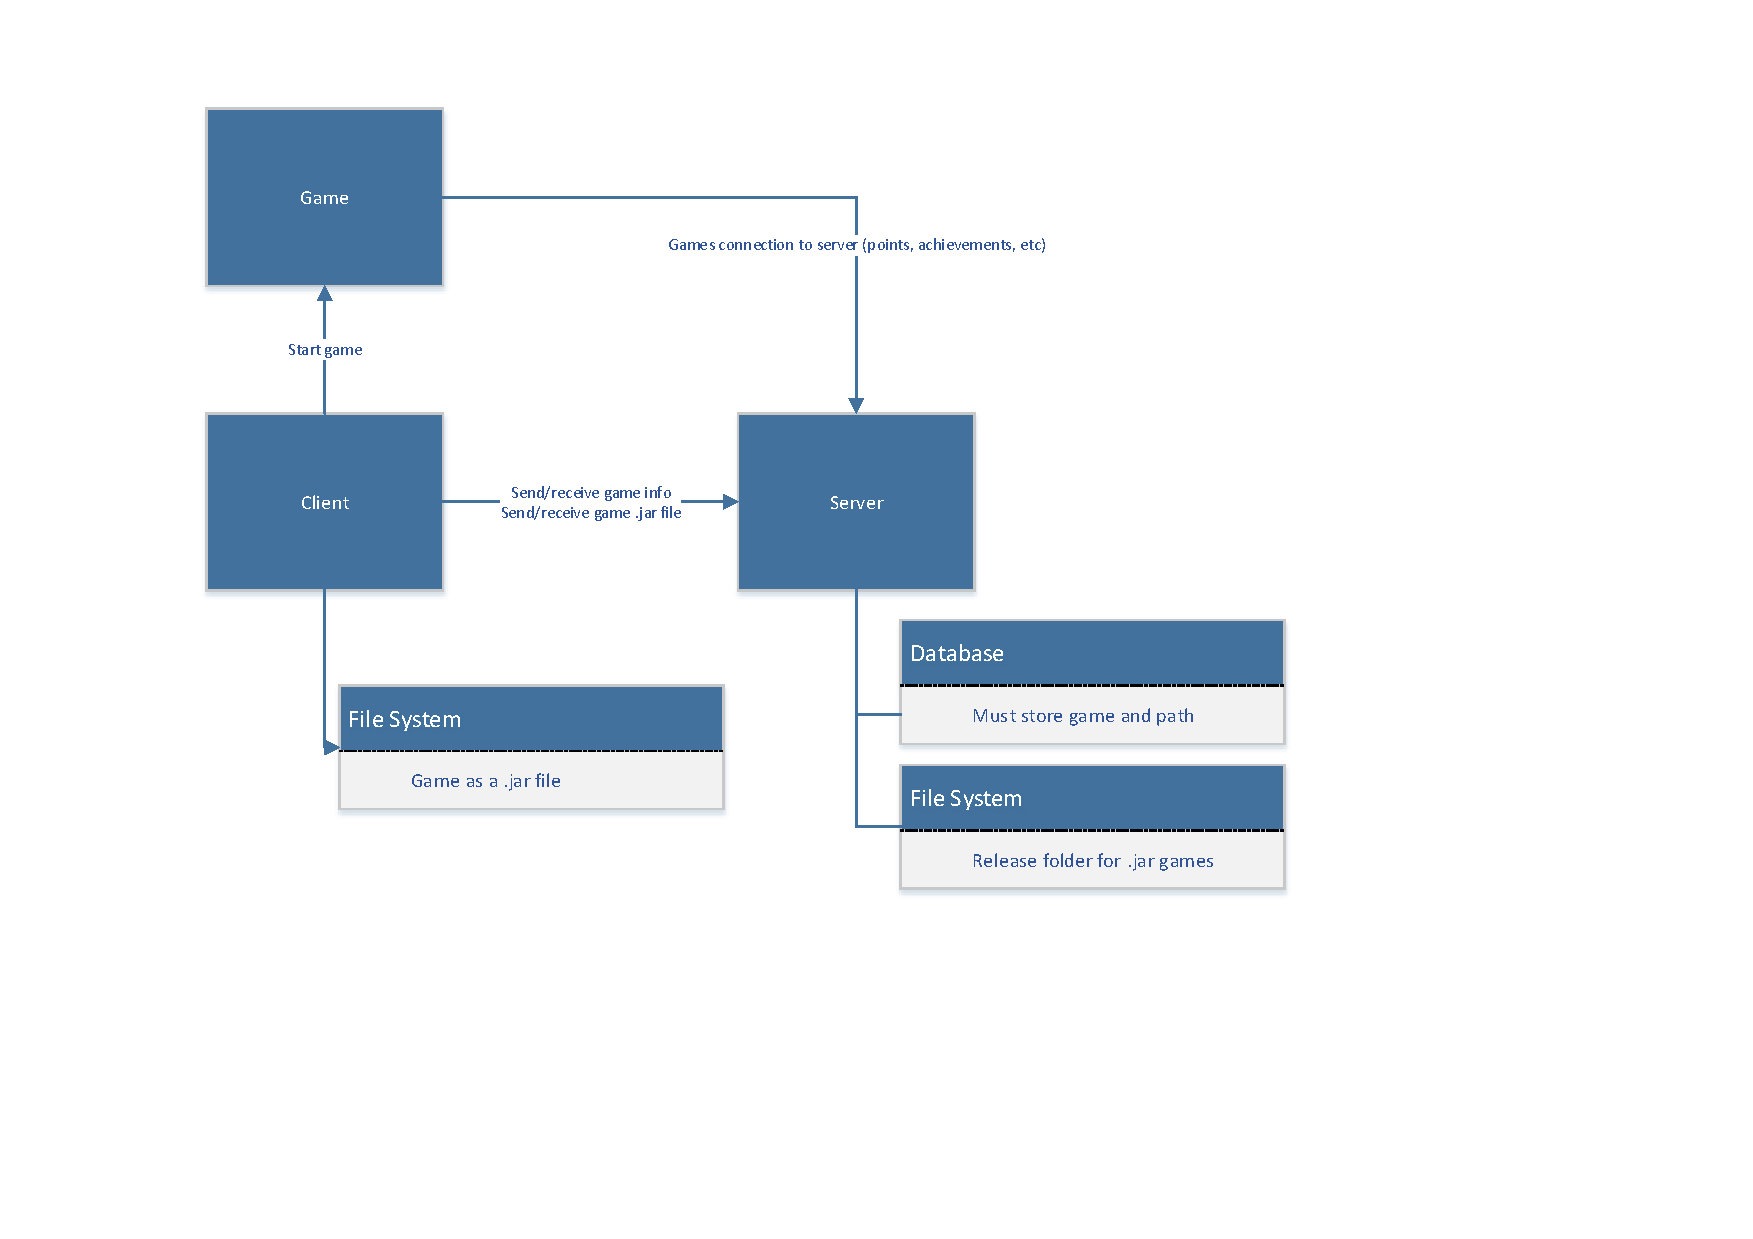
\includegraphics[trim=3cm 5cm 5cm 2cm,
                         clip=true,
                         width=\textwidth]{logarch.pdf}
    \end{figure}
    
\end{frame}

\section{Progress} %------------------------------------------------------------
\subsection{}

\begin{frame}
    \frametitle{Progress}
    
    Completed:
    
    \begin{itemize}
        \item   Understand current system (Reflection, Gradle tasks)
        \item   Determine architecture
        \item   Set up of server package manager
        \item   Set up of client package manager
        \item   Class paths read from text file
        \item   Pack games into .jars
    \end{itemize}
\end{frame}

\begin{frame}
    \frametitle{Progress}
    
    Being done now:
    
    \begin{itemize}
        \item   Package client connecting to package server
        \item   Populate release folder
        \item   Server setting up database connection
    \end{itemize}
\end{frame}

\begin{frame}
    \frametitle{Progress}
    
    To be done:
    
    \begin{itemize}
        \item   Interface with other groups
        \item   Fetch game from server
    \end{itemize}
\end{frame}

\section{Feedback} %------------------------------------------------------------
\subsection{}

\begin{frame}
    \frametitle{Feedback}
    
    \begin{itemize}
        \item   System interfaces
        \begin{itemize}
            \item   Will this affect your group negatively?
        \end{itemize}
        \item   System architecture
        \begin{itemize}
            \item   Are there any flaws or redundancies?
        \end{itemize}
        \item   Possible improvements?
        \begin{itemize}
            \item   What could be structured differently, or extra features?
        \end{itemize}
    \end{itemize}
\end{frame}


\end{document}